\documentclass[12pt, a4paper]{article}
% \usepackage{mathtools}
\usepackage{graphicx}
\usepackage{amsthm}
\usepackage{hyperref}
\usepackage{amssymb}
\graphicspath{{images/}}

\hypersetup{
    colorlinks=true,
    linkcolor=blue,
    urlcolor=cyan
}

\title{AP Macroeconomics Notes}
\author{Franklin Chen}
\date{22 Feburary 2024 - 21 May 2025}

\theoremstyle{definition}
\newtheorem{definition}{Definition}

\begin{document}
\maketitle
\newpage
% comment

\tableofcontents

\newpage

\section{Intro to Economics}
Corresponds to Chapter 2: "The Discipline of Economics."

\subsection{What is Economics?}

\begin{definition}[Economics]
    The study of resources and how to optimally use resources.
    Often to answer the question "Should we do \textit{A} or \textit{B} with this limited resource?"
\end{definition}

In this context, the word "resource" has a specific meaning.

\begin{definition}[Resource]
    Anything that can be used to produce a good or service.
    Every resoruce is classified into one of three categories:
    \begin{itemize}
        \item \textbf{Land}: natural resources. (Eg. crude oil, farmland, oceans)
        \item \textbf{Labor}: work people do to produce goods and services. (Eg. physical labor like building or sports, mental labor like professors)
        \item \textbf{Capital}: equipment used to produce goods or more resources. (Eg. factories, computers)
    \end{itemize}
\end{definition}

Economics is broken into two fields: \textbf{microeconomics} and \textbf{macroeconomics}.

\begin{definition}[Microeconomics]
    The study of economic problems faced at the individual level; individuals, families, and firms.
    Eg. "does this particular family save enough to provide for its future needs?"
\end{definition}

\begin{definition}[Macroeconomics]
    The study of economics problems faced at the national level; states, countries, and internationally.
    Eg. "should we allocate resources from national defense to education?"
\end{definition}

Sometimes, we may discuss \textbf{positive economics}: the scientific analysis of economics via the hypothesis-test-conclusion model.
Alternatively, we may discuss \textbf{normative economics}: the ethical analysis of economics- the way things \textit{should} be.

\subsection{Opportunity Cost and the PPF}

\begin{definition}[Opportunity Cost]
    The potential benefit lost from choosing one alternative over the other.
    For example, when you spend two hours studying, you lose two hours of relaxation.    
    Gains of the option not chosen - gains of the opportunity chosen = opportunity cost.
\end{definition}

In macroeconomics, opportunity cost is often quantative.
If a nation decides to spend more resources to produce a good A, they will "lose" the good B that could have been produced with the same resources.

\begin{figure}[ht] % h = where it appears in text
    \centering
    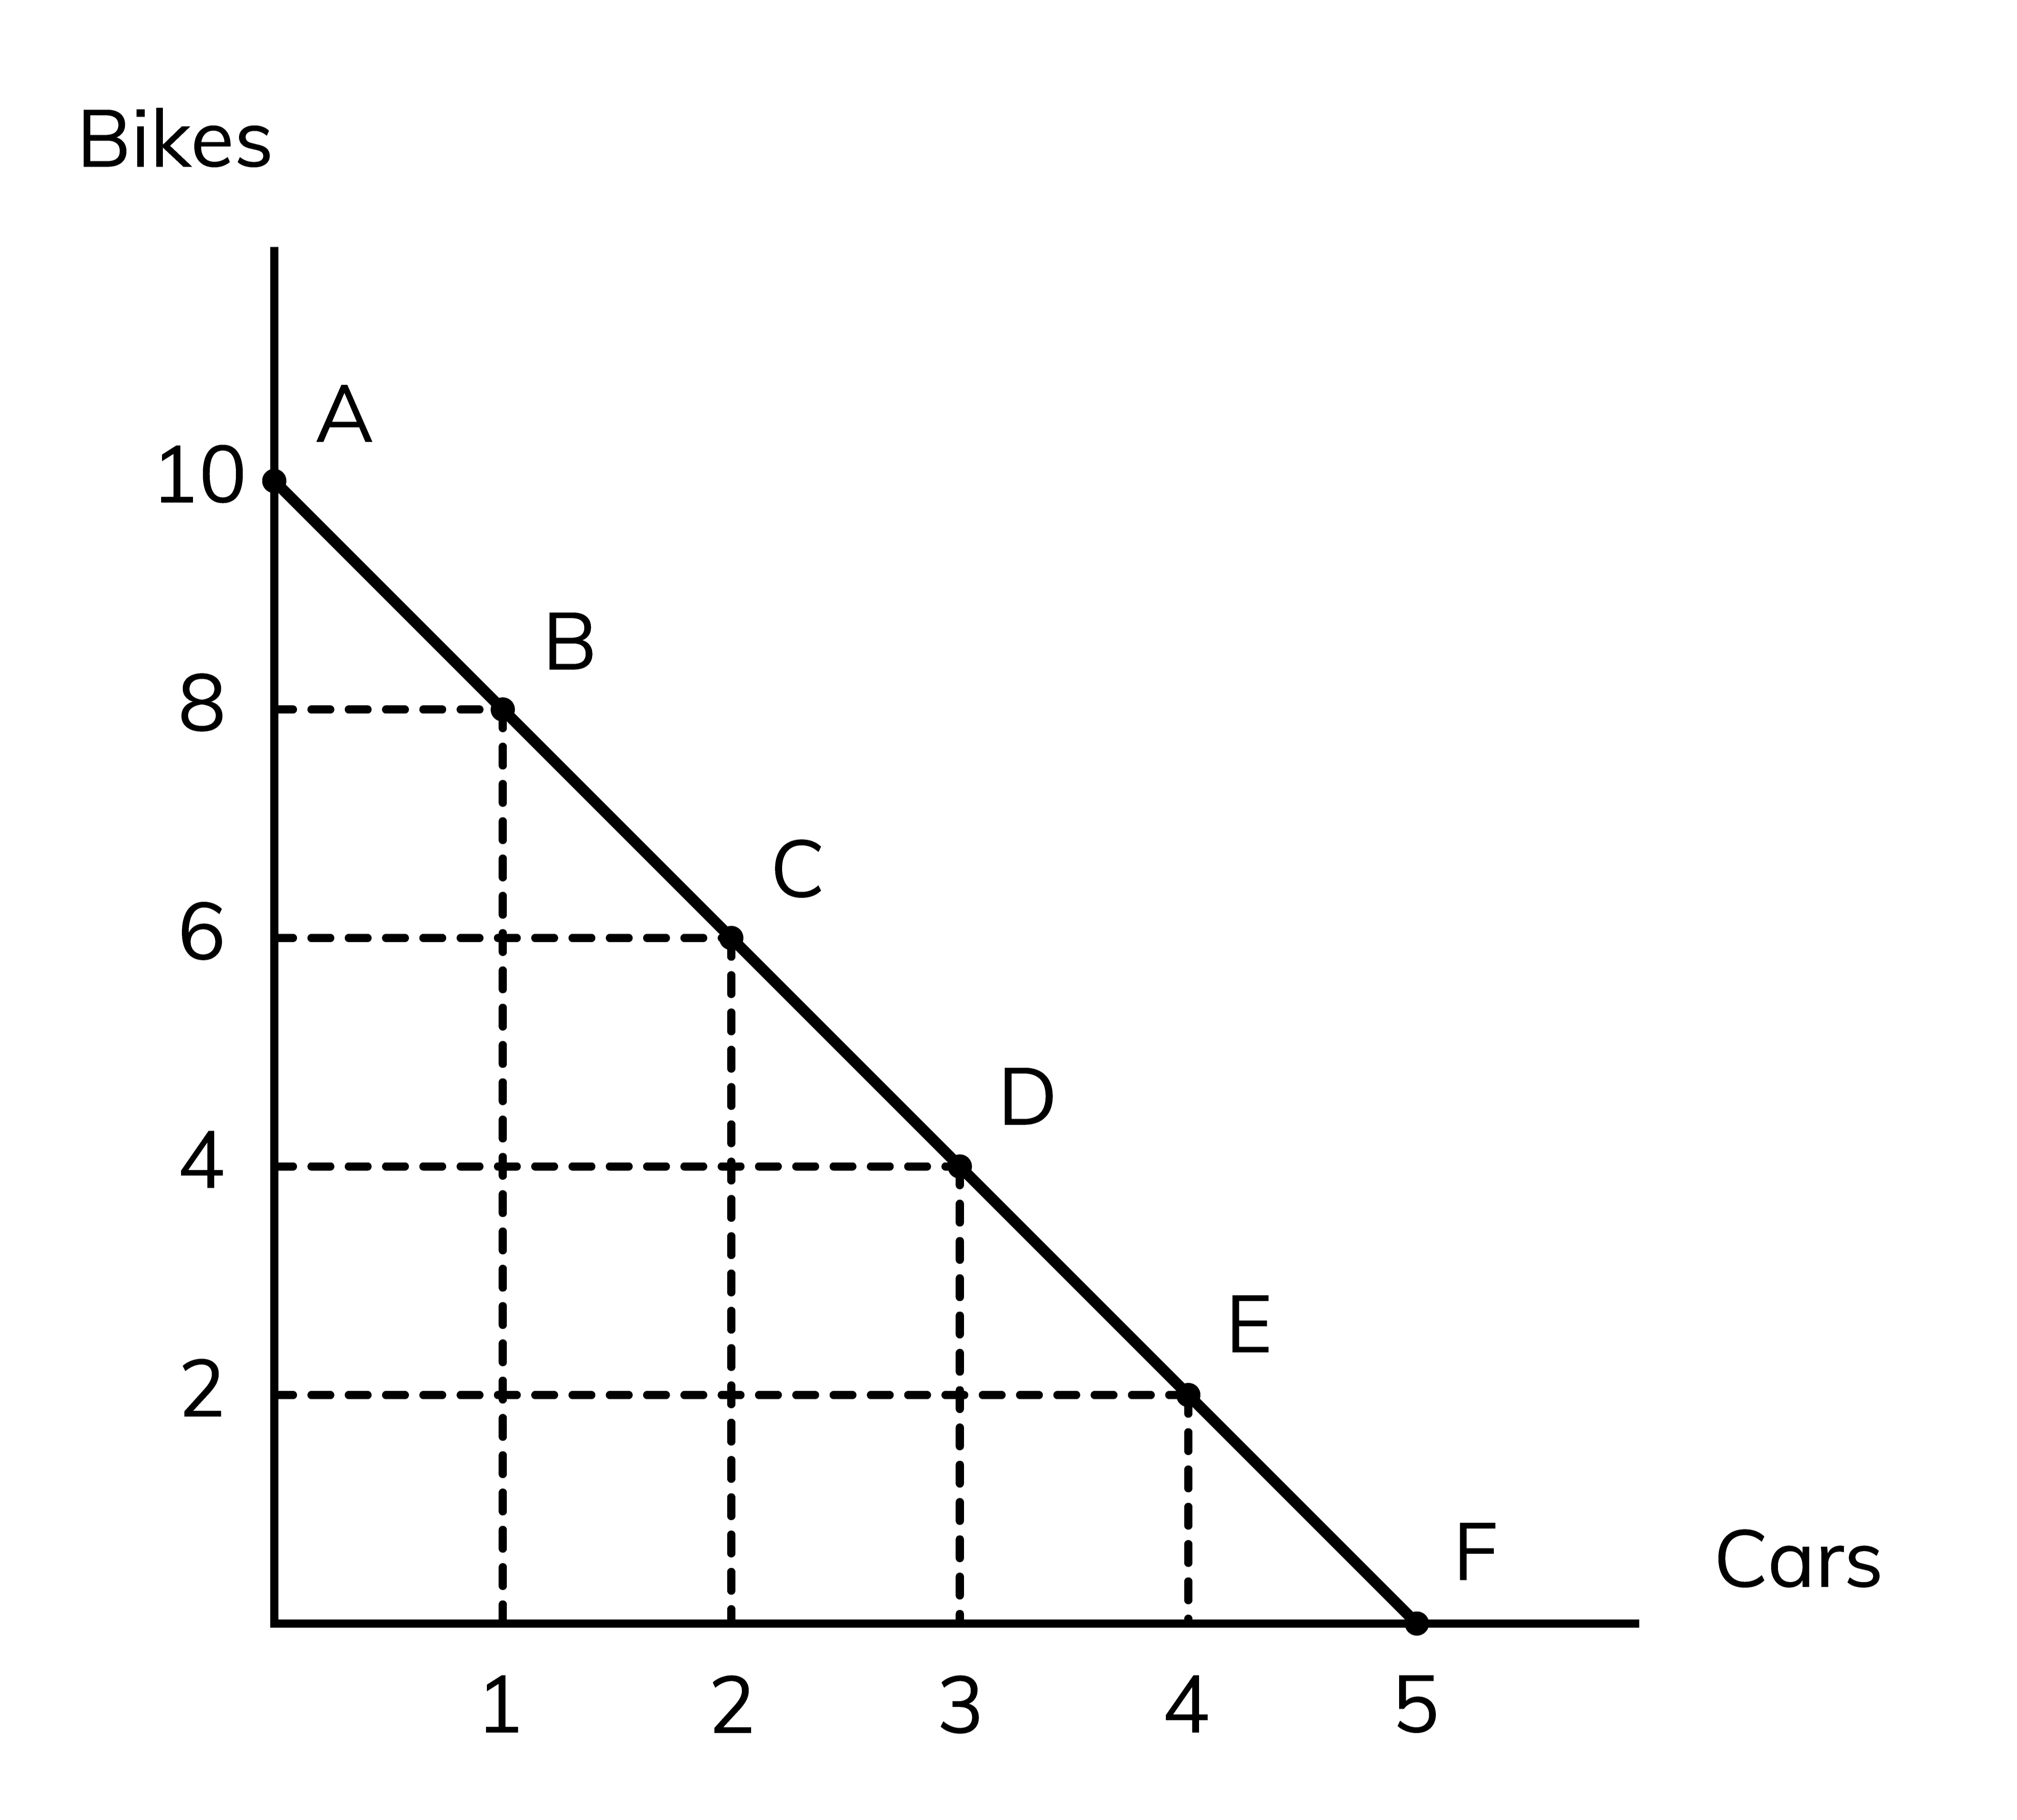
\includegraphics[width=0.75\textwidth]{ppf.png}
    \caption{A Production Possibilties Frontier (PPF) showing a hypothetical nation's possible production of bikes and cars.}
    \label{fig:ppf}
\end{figure}

For example, consider Figure \ref{fig:ppf}.
In this case:

\[\textrm{Opportunity Cost of Bikes} = \frac{\textrm{Change in Car Production}}{\textrm{Change in Bike Production}} = 0.5 \textrm{cars}/\textrm{bike}\]

The opporutnity cost of cars is the reciproical of the opportunity cost of bikes: that is, 2 bikes/car.

Figure \ref{fig:ppf} is a \textbf{production possibilties frontier}: it shows all the combinations of the goods that can be produced if the economy uses all of its resources fully and \textbf{efficently} (to their maximum potential).
\textit{All points on the curve are optimal; a normative analysis is required to determine what point is preferred.}

Points "inside" the PPF are possible, but aren't optimal. (This may occur due to environmental, labor or other restrictions.)
Points "outside" the PPF are currently impossible: resources can't be used efficently enough to reach that point.

The PPF may shift for two primary reasons: changes in the \textit{amount of resources} or \textit{productivity/technology}.
Increasing the amount of resources or improving technology used to produced said resources would shift the PPF to the right.
Similarly, decreasing the amount of resources or somehow regressing in technology (war/disaster) would shift the PPF to the left.


\subsection{Laws of Costs}
Often, PPFs aren't straight lines; the opportunity cost varies depending on the current amount being produced.
More often, the opportunity cost of each extra product increases per product already produced.
Graphically, this causes a PPF concave to the origin.
This is known as \textbf{the law of increasing costs}.

Generally, the law of increasing costs happens as people less and less in tune with producing a good are hired to produce it.

Alternatively, the inverse may happen: the opportunity cost of each extra product may decrease per product already produced.
This may happen as more infrastructure is put into place, it takes less resources to produce each unit good.
This causes a PPF convex to the origin, and is known as \textbf{the law of decreasing costs}.

\subsection{Absolute and Comparitive Advantage}
\begin{definition}[Specialization]
    When an entity focuses on the production of a limited scope of goods for greater efficency.
\end{definition}

It can be shown that dividing labor into specialized tasks could increase productivity and output, \textit{even at the national scale.}

\begin{figure}[ht] % h = where it appears in text
    \centering
    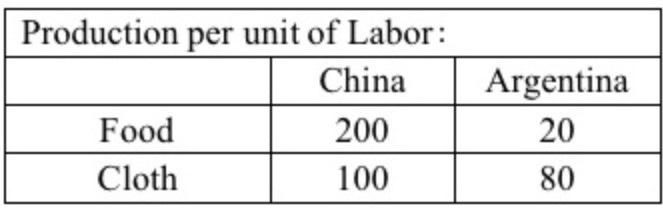
\includegraphics[width=0.75\textwidth]{advantage.jpg}
    \caption{A hypothetical example of production costs of food and cloth in China and Argentina.}
    \label{fig:advantage}
\end{figure}

Consider Figure \ref{fig:advantage}. 
In this case, China has the \textbf{absolute advantage} in both food and cloth because China can produce both more efficently than Argentina.
However, Argentina has the \textbf{comparitive advantage} in cloth, because it has a lower opportunity cost (0.25 food/cloth vs. 2 food/cloth).
Similarly, China has the comparitive advantage in food (0.5 cloth/food vs. 4 cloth/food).
It can be shown that by specializing in the good a nation has a competitive advantage of, the maximal amount of goods will be produced between the two nations.

Supposing that countries only produce their competitive advantage good, an optimal trading ratio to benefit both countries can be found by considering opportunity cost.
Trading x units of food for y units of cloth would be optimal if x/y is less than the opportunity cost of cloth in China (2 food/cloth) and y/x is less than the opportuntiy cost of food in Argentina (4 food/cloth).
For example, trading 1 unit of food per 1 unit of cloth would benefit both countries, as it is less than both of the countries' individual opportunity costs.

\newpage

\section{Economic Systems}
Corresponds to Chapter 3: "Economic Systems."

Economics deals with three primary problems:
\begin{itemize}
    \item How much, if any, of each good and service should be produced?
    \item Who will get how much of each good and service?
    \item How should these goods and services be distributed?
\end{itemize}

While these problems may be easy to answer for small systems, these problems become exponentially harder to deal with as the size of the economy grows.
Note the idea of opportunity cost (producing something will reduce production of other products) 
and \textit{related costs}: producing more of a product will require more production of capital.

For example, producing more food may take away money from the cosmetic industry; opportunity cost; and require the production of more tractors and farm equipment; related costs.

Societies tackle this problem in three ways: \textbf{command economies}, \textbf{capitalism}, or a mix of the two.
These can be viewed as a spectrum: command economies on one end, and capitalism on the other.

\subsection{Command Economies}
\begin{definition}[Command Economy]
    Also referred to as "communism" or "socialism."
    An economy in which the government determines what will be produced, how much will be produced, and who recieves the products.
\end{definition}

Command economies use quotas and production plans to dictate how much of each good or resource is produced. 
By setting prices on goods and services and controlling the wage rates of almost all citizens, the government is able to control the access to products.

Due to how interconnected individual goods and services are with one another, it is nearly impossible to perfectly coordinate production requirements.
Many quotas may fail if a "requirement" quota fails to be met.
Additionally, incentives to work hard and innovate are discouraged, as there is little benefit for doing so.

However, command economies can also artificially change prices; ex. artificially lowering the price of textbooks to encourage education.
Additionally, fixed wages can eliminate the lower class.

Two examples of countries with command economies are Cuba and North Korea.

\subsection{Capitalism}
\begin{definition}[Capitalism]
    Economic system where supply and demand determine prices.
\end{definition}

In a capitalist economy, the \textbf{consumer} dictates the production of goods.
For example, if consumers want more of a certain product, the purchases of that product will go up.
This signals to producers to increase the production of that product (often cutting something else in the process).

An individual's income determines how much of the net production they will recieve.
Income is also another variable within such an economy (the price of labor).

In a purely capitalist economy, the government has no direct influence.
However, in practice, no country is purely capitalist: the government often needs to step in when the economy won't equitably provide important resources, like food or higher education.

\subsubsection{Allocative Efficency}
\begin{definition}[Allocative Efficency, the "invisible hand"]
    When resources are deployed to produce just the right amount of products to satisfy society's wants.
\end{definition}


When prices are determined by a capitalist economy, \textbf{allocative efficency} is achieved.
The capitalist economy is able to answer the critical questions of economics in a \textit{decentralized} way (with no ruling body).
Products and quantity are determined by the consumer, as mentioned before.
Who recieves goods is also answered, as the price of labor will reward those who appeal to consumer wants.

\subsection{The Circular Flow Diagram}

\begin{figure}[ht] % h = where it appears in text
    \centering
    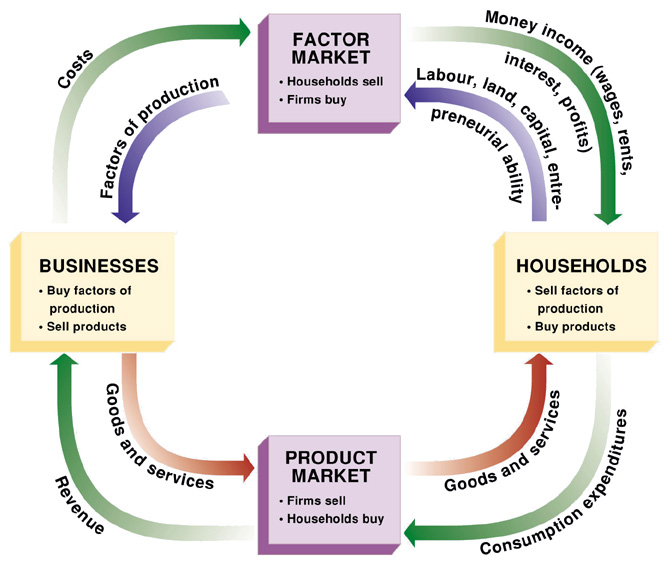
\includegraphics[width=0.75\textwidth]{circular flow.jpg}
    \caption{The Circular Flow Diagram.}
    \label{fig:cfd}
\end{figure}
In capitalist economies, most of the resources are "owned" by individuals and households;
via stockholders "owning" companies and government facilites being "owned" by everybody.

\begin{definition}[Market]
    A mechanism that allows buyers and sellers to exchange a good or service.
\end{definition}


The \textbf{circular flow diagram} (\ref{fig:cfd}) shows how resources are flow from households to firms in exchange for wages.
This trade of resources for money is known as the \textit{market for resources} or \textit{factor market}.
Households spend their income to purchase goods and services supplied by firms: the \textit{market for goods and services} or \textit{product market}.


\newpage

\section{Supply and Demand}
Correpsonds to Chapter 4: "Demand and Supply: The Basics."

\newpage

\section{National Economic Accounts}
Corresponds to Chapter 12: "The National Economic Accounts."

\newpage

\section{Inflation and Unemployment}
Corresponds to Chapter 13: "Inflation and Unemployment."

\newpage

\section{Money and Banking}
Corresponds to Chapter 14: "Money and Banking"

\newpage

\section{Monetary Theory}
Corresponds to Chapter 15: "Monetary Theory"

\newpage

\section{Aggregrate Supply and Demand}
Corresponds to Chapter 16: "Aggregrate Supply and Aggregrate Demand"

\newpage

\section{Monetary Policy}
Corresponds to Chapter 17: "Monetary Policy"

\newpage

\section{Fiscal Policy}
Corresponds to Chapter 18: "Fiscal Policy"

\newpage

\section{International Trade and Finance}
Corresponds to Chapter 19: "International Trade and Finance"

\newpage

\end{document}